%\documentclass{beamer}
\documentclass[handout]{beamer}
\usetheme{boxes} 
%\usetheme{default}

%math fonts
%\renewcommand\mathfamilydefault{\rmdefault}

%page numbers
\setbeamertemplate{footline}[page number]

\setbeamercovered{invisible}
\setbeamertemplate{navigation symbols}{} 
\usepackage{mathtools}
\usepackage{graphicx}
\usepackage{amsmath}
\usepackage{epstopdf}
\usepackage{color}


\title[Trajectory Tracking]{Optimizing Robot Striking Movement Primitives with Iterative Learning Control}
\author{Okan Ko\c{c}}
\institute[IAS]
{
MPI for Intelligent Systems, T\"ubingen \\
Robot Learning Lab \\
\medskip
{\emph{okan.koc@tuebingen.mpg.de}}
}
\date{\today}

% custom commands
\newcommand{\boldvec}[1]{\boldsymbol{\mathrm{#1}}}
\let\vec\boldvec
\newcommand\at[2]{\left.#1\right|_{#2}} % the at differential sign
\newcommand\scalemath[2]{\scalebox{#1}{\mbox{\ensuremath{\displaystyle #2}}}} % scaling matrices

%% custom macros
\newcommand{\todo}{\textcolor{red}{TODO}} % TODO!
\newcommand{\kin}{\mathcal{T}} % used to denote inverse kinematics
\newcommand{\invKin}{\mathcal{T}^{-1}} % used to denote inverse kinematics

\newcommand{\joint}{\vec{q}} % used to denote robot state in joint space
\newcommand{\state}{\vec{y}} % denotes the generalized coordinates - joint space and velocity coordinates
\newcommand{\dmp}{\vec{s}} % used to denote the dmp trajectory states
\newcommand{\error}{\vec{e}} % difference between state and reference
\newcommand{\traj}{\vec{r}} % used to denote the points on the trajectory to be tracked

\newcommand{\dist}{\vec{\epsilon}} % denotes the disturbances acting on the rigid body dynamics
\newcommand{\linDist}{\vec{d}} % denotes the disturbances on the LTV model

\newcommand{\sysInput}{\vec{u}} % used to denote the system inputs
\newcommand{\linInput}{\tilde{\sysInput}} % denotes the LTV inputs
\newcommand{\trjInput}{\sysInput_{\mathrm{IDM}}} % denotes the inputs on the trajectory (calculated using IDM)


% % % % DMP terminology % % % %
\newcommand{\fullvec}{\vec{\psi}} % full vector for state-ref-dmp-goal
\newcommand{\goal}{\vec{g}} % goal state
\newcommand{\force}{\vec{f}} % forcing term of the dmps
\newcommand{\phase}{x} % phase of the dmp
\newcommand{\weights}{\vec{w}} % weights of the dmp
\newcommand{\basis}{\vec{\Phi}} % basis functions of the dmp as a matrix

% % % % ILC terminology % % % %
\newcommand{\qmatrix}{\vec{\Gamma}} % denotes the filtering qmatrix term of Bristow et al.
\newcommand{\lmatrix}{\vec{L}} % denotes the learning matrix of Bristow et al.

\newcommand{\dynamics}{\vec{f}}
\newcommand{\dynamicsNominal}{\dynamics_{\mathrm{nom}}}
\newcommand{\policy}{\vec{\pi}}
\newcommand{\ValueFunction}{J}
\newcommand{\episode}{k} % used for episode number

\newcommand{\totalTime}{T} % total time duration 
\newcommand{\numSteps}{N} % total number of time steps
\newcommand{\numepisode}{K} % total number of episodes

\newcommand{\threshold}{\epsilon}
\newcommand{\alg}{\emph{wILC}}
\newcommand{\dataset}{E}

% Set the paths where all figures are taken from:
\graphicspath{{Pictures/}}
\mathtoolsset{showonlyrefs} 
\newcommand{\includesvg}[1]{%
% \executeiffilenewer{#1.svg}{#1.pdf}%
% {inkscape -z -D --file=#1.svg %
% --export-pdf=#1.pdf --export-latex}%
 \input{#1.pdf_tex}%
}

\begin{document}
%
\begin{frame}
\titlepage
\end{frame}
%
\begin{frame}
\frametitle{Table of Contents}
\tableofcontents
\end{frame}
%
\section{Motivation}
%
\begin{frame}{Setup}
\begin{itemize}
\item In order to hit the ball to a desired position on the opponent's court, we give the robot reference trajectories that facilitate the right striking motion. We can teach the robot such trajectories via kinesthetic teach-in.
\end{itemize}
\begin{figure}[b!]
\center
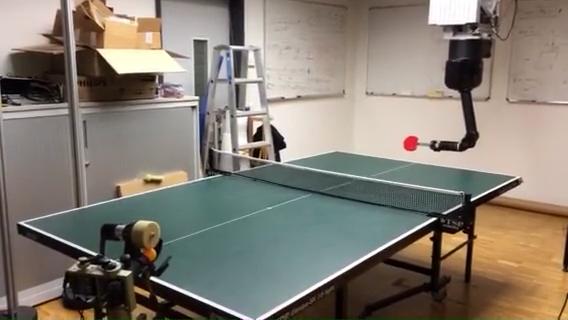
\includegraphics[scale=0.4]{robot1.png}			
\label{robot}
\end{figure}
\end{frame}
%
\begin{frame}{Movement Primitives}
\begin{itemize}
\item Dynamic Movement Primitives (DMP) are a dynamical systems based approach to represent reaching motions:
\begin{equation}
\begin{aligned}
\dot{\dmp} &= \vec{A}_s \dmp + \basis(\phase) \weights,
\label{dmp2}
\end{aligned}
\end{equation}
\item Approximation and control errors in table tennis make the application of DMPs less useful in practice. Small changes to DMPs can often make them more useful.
\end{itemize}
\end{frame}
%
\begin{frame}{Research Question}
\begin{itemize}
\item How can we execute optimally hitting movement primitives either in table tennis or a similar reaching task e.g., putting in golf. 
%
\item More specifically, when we have modelling inaccuracies, how should we modify a DMP $\dmp(t)$ such that the robot executes a desired hitting motion?
\end{itemize}
\end{frame}
%
\begin{frame}{Iterative Learning Control (ILC)}
\begin{itemize}
\item Task: track a reference trajectory $\traj(t), \ 0 \leq t \leq T \ $ under unknown repeating disturbances or model mismatch.
\item Feedforward control inputs $\sysInput(t)$ are adjusted after each iteration. The goal is drive the deviations from the trajectory to zero. 
\end{itemize}
\begin{figure}
\center
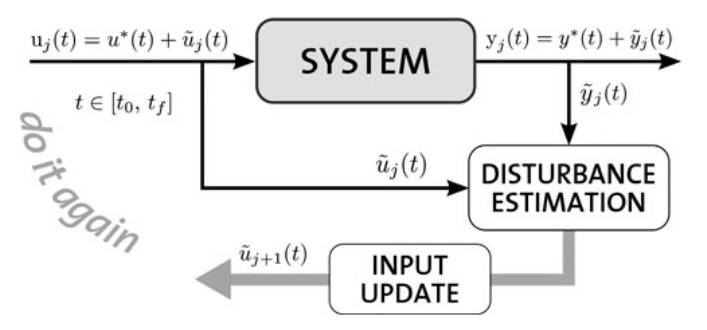
\includegraphics[scale=0.25]{ilc_framework}			
\caption{ILC Framework}
\end{figure}
\end{frame}
%
%
\begin{frame}{Iterative Learning Control (ILC)}
\begin{itemize}
\item For a linear system $\dot{\state}(t) = \boldvec{A}(t)\state(t) + \boldvec{B}(t)\sysInput(t)$,
\item A very simple update rule is to use the error $\error_k = \state_k - \traj$ and its derivatives. For example:
\begin{equation*}
\begin{aligned}
\sysInput_{k+1} = \sysInput_{k} + K_{p}\error_k + K_{d}\dot{\error}_k
\end{aligned}
\end{equation*}
\item It can easily lead to unstability! Model based update laws can be much more effective in practice!
\end{itemize}
\begin{figure}
\center
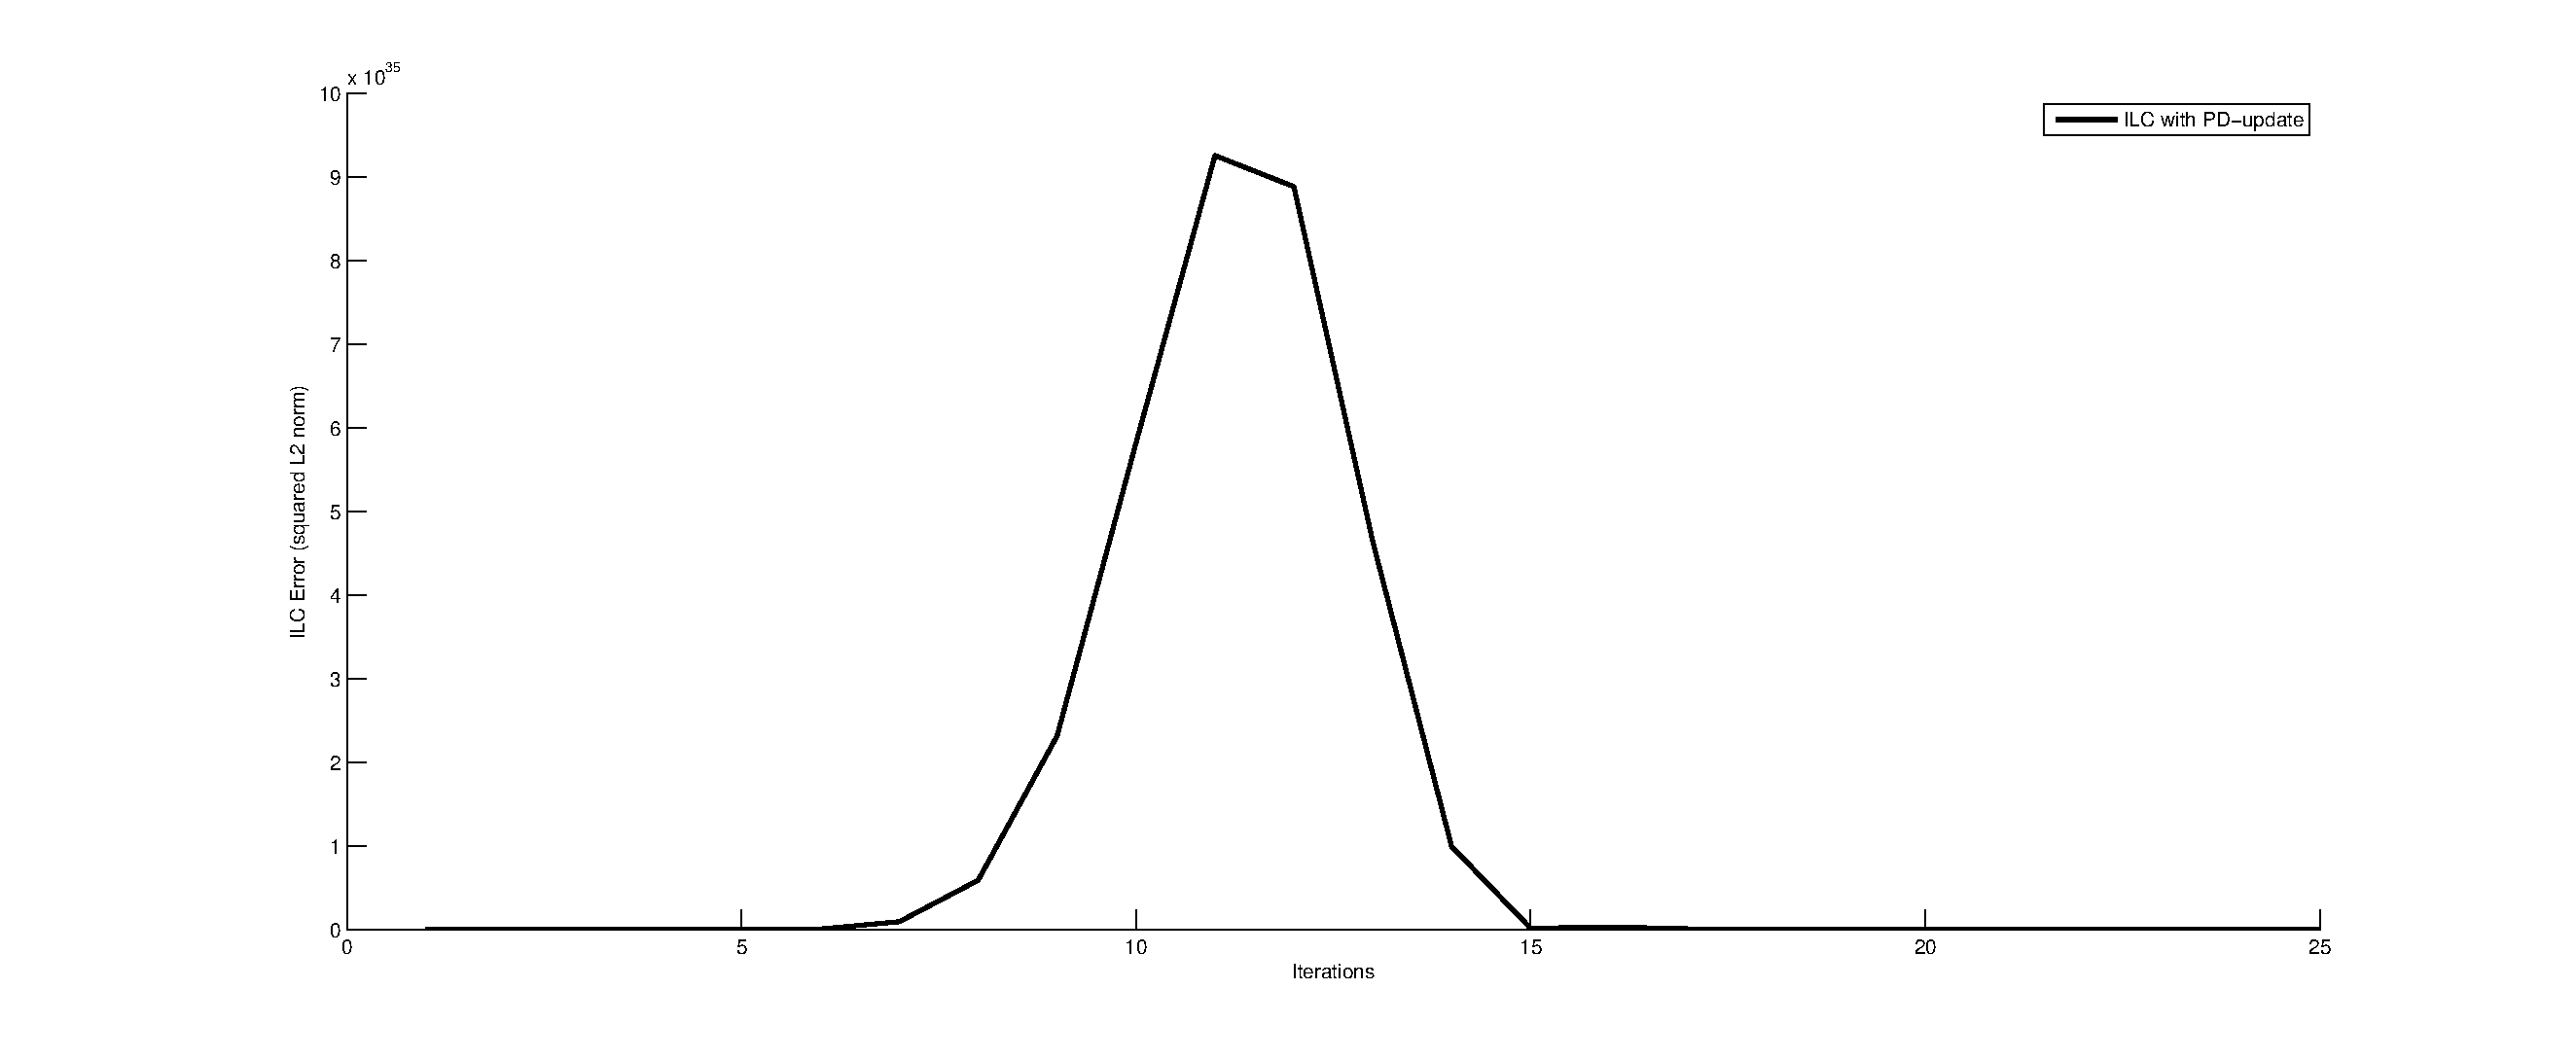
\includegraphics[scale=0.2]{ilcBlowup}			
\caption{Naive ILC Implementation}
\end{figure}
\end{frame}
%
\begin{frame}{Generic ILC Update Rule}
\begin{itemize}
\item ILC update rules can be written as: $\sysInput_{k+1} = \qmatrix(\sysInput_{k} - \lmatrix\error_{k})$
\item Using the cost functional $J(\sysInput) = \sum_{j=1}^{T} \error_j^{\mathrm{T}}\vec{Q}\error_j + \sysInput_j^{\mathrm{T}}\vec{R}\sysInput_j$ as our optimality criterion,
\item Newton's method gives us a model-based ILC update rule: 
\end{itemize}
\begin{equation*}
\begin{aligned}
\lmatrix &= (\vec{F}^{\mathrm{T}}\vec{Q}_L\vec{F} + \vec{R})^{-1}\vec{F}^{\mathrm{T}}\vec{Q}_L \\
\vec{F}_{(i,j)} &= \left \{
\begin{array}{cc}
\vec{A}_{i-1}\ldots \vec{A}_j\vec{B}_{j-1}, & j < i \\ 
\vec{B}_{j-1}, & j = i \\
\vec{0}, & j > i 
\end{array} \right.
\end{aligned}
\end{equation*}
\end{frame}
%
\begin{frame}{ILC with Movement Primitives}
\begin{itemize}
\item Equivalently we can update the DMP weights $\weights_k$ if we have feedback on our system.
\end{itemize}
\begin{figure}
\center
\includegraphics[scale=0.5]{fb_plant}			
\caption{Inputs to the feedback coupled system is now $\dmp(t)$.}
\end{figure}
\end{frame}
%
\section{Methodology}
%
\begin{frame}{Problem Setting}
\begin{itemize}
\item Problem: Continuous time trajectory tracking under the \emph{nonlinear} system dynamics: 
\end{itemize}
\begin{equation*}
\begin{aligned}
\dot{\state}(t) &= \mathbf{f}(\state(t),\sysInput(t)) \\
\end{aligned}
\end{equation*}
\begin{itemize}
\item Goal: Track a reference trajectory $\traj(t), \ 0 \leq t \leq T \ $ by applying the control inputs $\sysInput^{*}(t)$. 
\item Use: Any trajectory generation algorithm.
.
\end{itemize}
\end{frame}
%
\begin{frame}{Problem Setting}
\begin{itemize}	
\item However $\mathbf{f}$ is not known very well! 
\item We will fail to track $\traj(t)$ just by applying $\sysInput^{*}(t)$.
\item We can use ILC to correct for deviations! 
\end{itemize}
\end{frame}
%
\subsection{Lifted vector representation}
%
\begin{frame}{Linearize Around Trajectory}
\begin{itemize}
\item Linearize model around trajectory: 
\end{itemize}
\begin{equation*}
\begin{aligned}
\dot{\state}(t) &= A(t)\state(t) + B(t)\sysInput(t) \\
\end{aligned}
\end{equation*} 
\begin{itemize}
\item The time variant matrices are: 
\linebreak
\end{itemize}
\begin{equation*}
\begin{aligned}
A(t) & = \at{\frac{\partial{\mathbf{f}}}{\partial{\state}}}{(\state^{*}(t),\sysInput^{*}(t))} \\
B(t) & = \at{\frac{\partial{\mathbf{f}}}{\partial{\state}}}{(\state^{*}(t),\sysInput^{*}(t))} \\
\end{aligned}
\end{equation*}
\end{frame}
%
\begin{frame}{Discretize linearized model}
\begin{itemize}
\item For k $\in \{ 0, 1, \ldots, N-1 \}$, 
\end{itemize}
\begin{equation*}
\begin{aligned}
\state(k+1) &= A_{D}(k)\state(k) + B_{D}(k)\sysInput(k) \\
\end{aligned}
\end{equation*}

\begin{itemize}
\item The discretized matrices can be found using: 
\linebreak
\end{itemize}
\begin{equation*}
\begin{aligned}
\exp^{h
\left[
\scalemath{0.5}{
\begin{array}{c|c}
A(k) & B(k) \\ \hline
0 & 0
\end{array}}\right]}
&= 
\left[
\begin{array}{c|c}
A_{D}(k) & B_{D}(k) \\ \hline
0 & I
\end{array}\right] \\
C_{D}(k) &= C(k)
\end{aligned}
\end{equation*}
\end{frame}
%
\begin{frame}{Lifted Vector Representation}
\begin{itemize}
\item Stack inputs together, $\sysInput_L = (\sysInput(1), \ldots, \sysInput(N-1))$ to obtain the lifted vector form: 
\end{itemize}
\begin{equation*}
\begin{aligned}
\state_L &= F\sysInput_L + d_L \\
\end{aligned}
\end{equation*}

\begin{itemize}
\item where the submatrices are: 
\linebreak
\end{itemize}
\begin{equation*}
\begin{aligned}
F_{(i,j)} &= \left \{
\begin{array}{cc}
A_{D}(i-1)\ldots A_{D}(j)B_{D}(j-1), & j < i \\ 
B_{D}(j-1), & j = i \\
0, & j > i 
\end{array} \right. \\
G_{(i,j)} &= C_{D}
\end{aligned}
\end{equation*}
\end{frame}
%

%
% End of slides
% TODO: add supplementary material!
\end{document} 